\anexo{Cronograma de Proyecto}

\section*{A.1 Diagrama de Gantt}
\addcontentsline{toc}{subsection}{A.1 Diagrama de Gantt}

El siguiente cronograma presenta la planificación pormenorizada del proyecto, organizada en cuatro fases principales con un total de veinte tareas distribuidas a lo largo del período marzo--diciembre de 2026. La granularidad adoptada es quincenal, identificando cada período como S1 (primera quincena) y S2 (segunda quincena) dentro de cada mes. Para cada tarea se especifica su tarea predecesora en la columna ``Dep.'', lo que permite visualizar las dependencias técnicas entre actividades y evaluar el impacto de eventuales desvíos sobre la ruta crítica del proyecto.

\begin{figure}[ht]
    \centering
    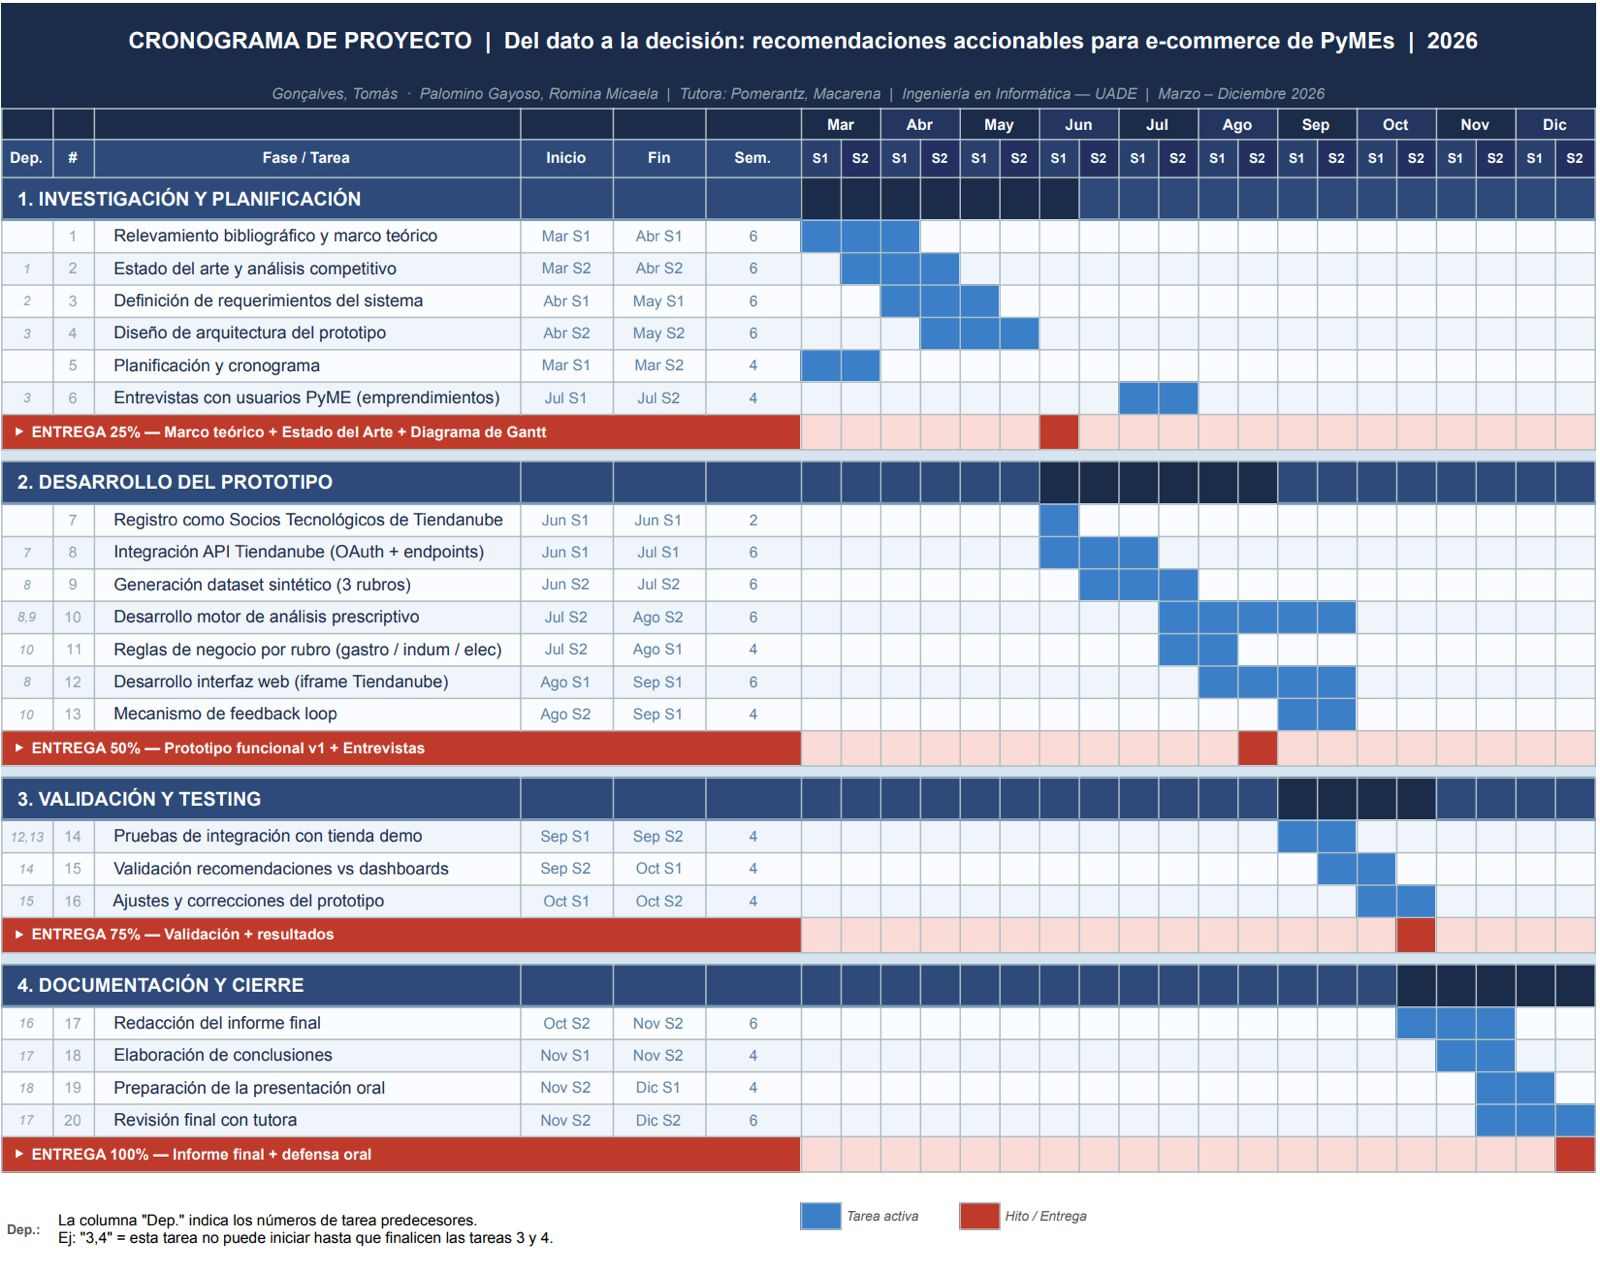
\includegraphics[width=\textwidth]{./gantt/gantt_pfi_palominoGoncalves.jpeg}
    \caption{Cronograma de proyecto --- Diagrama de Gantt.}
\end{figure}

\noindent\textit{Fuente: elaboración propia. El archivo editable con detalle quincenal completo se encuentra disponible en \href{https://docs.google.com/spreadsheets/d/1RAgiah4WoOmxSgkorFZD4-IMevJZzECZ6DJtNFgUqrY/edit?usp=sharing}{este enlace (Google Sheets)}.}

\section*{A.2 Justificación técnica de desvíos anticipados}
\addcontentsline{toc}{subsection}{A.2 Justificación técnica de desvíos anticipados}

Al momento de la presente entrega (25\%), el proyecto se encuentra dentro de los plazos planificados. No obstante, se identifican a continuación los principales riesgos de desvío temporal, junto con las estrategias de mitigación previstas para cada uno.

\bigskip
\noindent\textbf{Desvío potencial 1 --- Registro como Socia Tecnológica de Tiendanube (Tarea 7)}

El proceso de registro en el programa de Socios Tecnológicos de Tiendanube es un prerrequisito directo para las tareas de integración con la API (Tarea 8) y, en cascada, para el desarrollo del motor de análisis (Tarea 10) y la interfaz web (Tarea 12). En caso de que los tiempos de aprobación por parte de Tiendanube superen los estimados, se adelantará el desarrollo del dataset sintético (Tarea 9), que puede ejecutarse de forma independiente, evitando así el bloqueo de la ruta crítica del desarrollo.

\bigskip
\noindent\textbf{Desvío potencial 2 --- Entrevistas con usuarios PyME (Tarea 6)}

La concreción de entrevistas con propietarios de emprendimientos y comercios de pequeño y mediano tamaño depende de la disponibilidad de terceros, lo que introduce incertidumbre en su planificación. Por esta razón, las entrevistas se planificaron para la primera quincena de julio, con margen suficiente para ser incorporadas en la entrega del 50\% en caso de no completarse en la fecha prevista.
